\documentclass{article}
\usepackage[utf8]{inputenc} 
\usepackage{amsmath}
\usepackage{amssymb}
\usepackage{wrapfig}
\usepackage{graphicx}
\usepackage{hanging}
\usepackage{float}
\usepackage[a4paper, total={6in, 8in}]{geometry}

\graphicspath{{./figures}}


\title{IMCS Project I Final Report}
\author{Travis Durrant and Timothy Weathers}
\date{December 4th, 2024}
\begin{document}
\maketitle
\subsection*{1.1: Introduction}
Machine learning is currently unique in the area of computer science in the sense that it offers many opportunities in one. It is a topic at the forefront of the modern cultural zeitgeist, due in no small part to the influence of ChatGPT and other large language models. Machine learning is also very easy to get into because of the availability and ease of use of various libraries dedicated to the purpose.

In this report, we will explore a classical beginner’s example of machine learning, the MNIST digit classification problem. This problem is an example of multi-label image classification, and is a good starting point for programmers new to machine learning.

We will be using the python TensorFlow library to handle the programming aspect of this project. TensorFlow has the advantage of handling most of the mathematical importance - and thus hiding it from not just the user, but the programmer as well. We will regardless spend some time exploring the mathematical background, and a few of the underlying algorithms that make machine learning work.


This report will assume the reader has an understanding of elementary linear algebra; a familiarity with the concept of matrices, matrix products, and the difference between vectors and scalars. An understanding of functions and calculus will prove useful as well, but we will not be touching on these topics in excessive detail.
\\
\subsection*{1.2: Problem Statement and Challenges}
We spoke briefly of the problem, calling it a multi-label classification problem. To explain this in even more detail, we describe our expected data and our target. These can also be thought of as the expected input, and expected output. The data we expect to be taking is an image, centred, padded, and grayscaled, that depicts a single digit on the range of $\{0,1,\cdots,9\}$. The desired target is the actual digit, in numeric form.

Since we expect a computer to take this image as input, and produce the numeric output, the challenge is then developing the program which does this. Even more formally, we need an algorithm of the following form: 
\[f: Image \rightarrow \{0,1,...,9\}\]

As can be expected, this algorithm will fall somewhere under the machine learning umbrella. Now, we will begin to look at the background required to make sense of the algorithm we will develop.
\\
\subsection*{2.1 Mathematical Background}
Machine learning is a very math-heavy exercise, despite usually falling under the umbrella of computer science. There are a few appropriate interpretations of a model. It can be viewed as a function, or a combination of functions, which is the approach we will take. There are other interpretations which view a model as a kind of statistical predictor: a “guessing machine”. This is not incorrect, and in fact we will take a cursory glance at a probability distribution to define our loss function later. Given we want a specific label though, we are not content with a probability distribution, and will take the highest predicted probability to be the model’s “answer” to our question.
\\
\subsection*{2.1.A Neurons}
A neuron is not quite the simplest machine learning element (that distinction belongs to the perceptron) but it is the first of which we are interested in. For the purpose of this report, we will think of a neuron as a function. It takes some input $x$, and produces some scalar output, $y$. Let’s look at the pieces of a neuron, and introduce some terminology.\\\\
\begin{figure}[H]
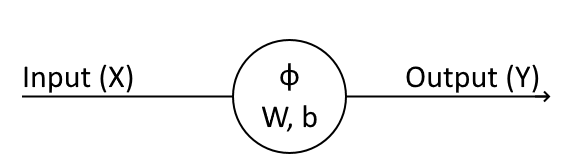
\includegraphics[width=\textwidth]{diagrams/neuron}
\caption{Visual representation of a neuron}
\end{figure}
$\phi$: This is the activation function. It is the most important piece to determine what a neuron does. Note that the anonymous signature of $\phi$ is as follows:
\[\phi: \mathbb{R} \rightarrow \mathbb{R}\]
$W$: This is called the weight. It is associated with the input $x$ by an anonymous product, that we denote as $<W, x>$. $W$ might be a scalar, if $x$ is a scalar. $W$ might also be a matrix, if $x$ is not a scalar. Either way, $<W,x>$ must be a scalar.\\\\
$b$: This is the bias. It is a value associated with the anonymous product by a simple sum. Bias is always a scalar.\\\\
The full behaviour of a neuron is given as:
\[y = \phi( <W,x> + b )\]

Neurons have one glaringly obvious limitation in that their range is always restricted to $\mathbb{R}$. This restriction may seem incredibly detrimental to their potential use cases. We will see, though, that clever combinations of neurons can lead to increasingly complicated behaviour.
\\
\subsection*{2.1.B Layers}
A layer, in the most general possible sense, is a function. In a more useful sense, it is a collection of neurons that collectively provide the output of the layer, and are provided input by some rule specific to the layer. In practice, a machine learning model is usually a series of sequentially applied layers. We will introduce some terminology first, and then explore some useful types of layers. First, the idea of a connection between neurons is very important when taking sequences of layers. When we say that two neurons are connected, it means that the output of the neuron in layer $n-1$ is provided as part of the input to a neuron in layer $n$. Second, to expand on the notion of sequential layers, we think of them as functions. Assuming the output space of layer $n-1$ corresponds to the input space of layer $n$, we can first apply layer $n-1$, and then layer $n$. They are applied sequentially. Now, to speak on three specific types of layers. We will introduce them, speak on their construction, and then list some advantages and disadvantages.\\\\

First of the three layers we care about is the dense layer - also sometimes referred to as a fully-connected layer. In a dense layer, every neuron belonging to the dense layer is connected to every neuron in the previous layer. These layers have the key advantage of being simple. There is no worry about input-output space match, because it is forced to match by the construction of the layer. The key disadvantage tied to this, is a flattening of the data. A dense layer, because of the full connection, “flattens” the data down to some $\mathbb{R}^n$. Any additional information that would be pulled out of positional information is lost. To illustrate this, imagine our output layer provides a sparse, banded matrix with some zeroes on the diagonal. This would be exceedingly hard for the dense layer to make meaningful sense of, because it “flattened” the data, and has only a long vector to work with.\\\\
\begin{figure}[H]
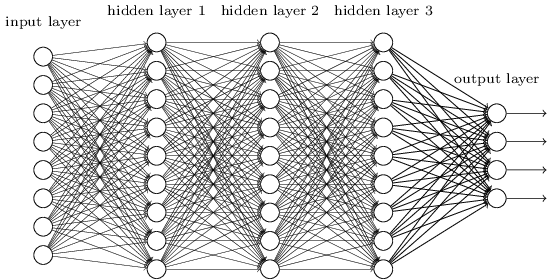
\includegraphics[width=\textwidth]{/diagrams/nielsendenselayer}
\caption{Visual representation of multiple dense layers (Nielsen 2019)}
\end{figure}

Second of the layers we need is formally referred to as a convolutional layer, also less formally a feature layer. A convolutional layer, in contrast to a dense layer, is not flat. It can be thought of as a grid in two dimensions - possibly more, but two dimensions is easy to visualize and works fine for our application. The way output is provided by this layer is as follows. First, a neighbourhood is defined, usually of a square size. We start by positioning this neighbourhood square in the top left corner. Using some activation function $\phi$, some weight $W$, and some bias $b$, a scalar is created which serves as output, and is connected to a single neuron on the next layer. This neuron is in the top left corner of our next grid. We take one step to the right, which may not move the square by exactly one neuron, if we pick a stride greater than one. This next output is connected to a neuron one space to the right of the previous. Rinse and repeat this process, to obtain all of the outputs that connect to the next layer. Note that, though it may seem counterintuitive, the weight matrix and bias remain constant across the layer. This is a requirement, so that the convolutional layer “looks for” the same pattern across the entire layer.
\begin{figure}[H]
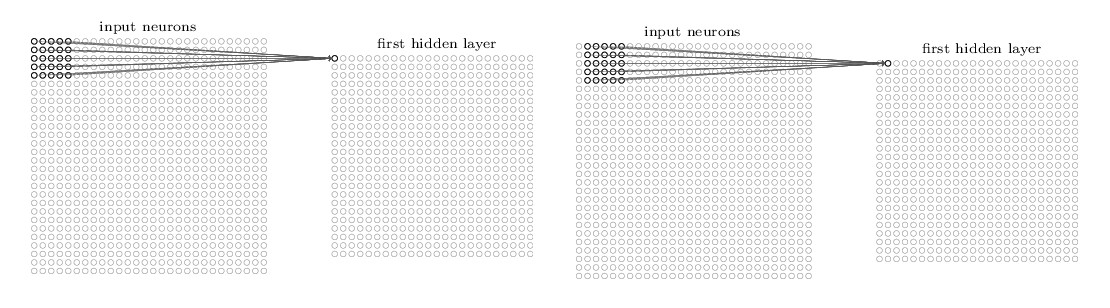
\includegraphics[width=\textwidth]{/diagrams/nielsenconvolutionlayer}
\caption{A convolutional layer with neighbourhood $5$x$5$ and stride of $1$ (Nielsen 2019)}
\end{figure}

The key advantage of the convolutional layer is positional relevance. As a result of the way the layer functions, key positional information is not flattened from the data with an elegance resembling the proverbial bull in a china shop. Note that a feature of the layer’s design, which often works out to be an advantage, is that it reduces the dimension of the data. At least, it does provided we don’t define neighbourhood size and stride both equal to one. The core disadvantage of this type of layer is the complication. There are a lot of hyperparameters to the layer (the nomenclature of which we will discuss later) which need to be picked in advance of the layer’s placement in a machine learning model. These are the neighbourhood size, and the stride. Often, these will be picked to help the dimensions of input-output spaces match as required, which proves to be another layer of complexity. When we put multiple convolutional layers together in parallel, we refer to the collection of parallel layers as the convolutional layer, and individuals as filters. We will be doing this.\\\\

The final layer we will discuss is referred to as a max-pooling layer. This type of layer works very similarly to the convolutional layer, with neighbourhoods being connected to a neuron on the next layer. The core difference is that we take the maximum of the neighbourhood as the output, rather than performing much actual computation to find the output. Note again the reduction in dimension, the same as a convolutional layer. Rather than positional data though, the purpose of a max-pooling layer is to provide translational invariance. For example, if all of the convolutional layer’s outputs were shifted one connection down on our visualization grid, the output of the max-pooling layer would barely change. Assuming, of course, we’ve picked a neighbourhood with size greater than one.\\
\begin{figure}[H]
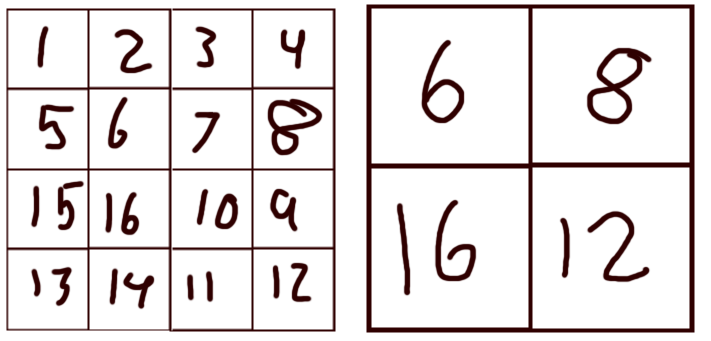
\includegraphics[width=\textwidth]{/diagrams/maxpooling}
\caption{A max-pooling layer with neighbourhood $2$x$2$ and stride of $1$}
\end{figure}

\subsection*{2.1.C Important Functions}
That was a lot of dense information about layers, so now we will take a quick look away, and discuss important functions that will be required for our methods. First, we look at the general concept of the loss function. In words, a loss function defines a distance between any two possible elements of the output space. The objective of most machine learning algorithms is to optimize the loss function to be as small as possible, by making changes to the parameters of the model. We’ll look specifically at an algorithm referred to as sparse categorical cross-entropy, which we will use as our loss function later, when we define the model. This defines a measure of difference between two different probability distributions.

\[Loss = -\sum_{i=0}^{9}p(x_i)\cdot \log \hat p(x_i) \]
In this case, we have explicitly adjusted the bounds of the sum to match our labels. $p(x)$ represents the true probability distribution, so in this case, it would be defined as  $1$ for the expected label, and $0$ otherwise. $\hat p(x)$ is also a discrete probability distribution, but it is the output of the model.\\\\

A softmax activation function, for our purposes, describes a confidence for each potential label (given the specific image input). All these confidences, by design of the function, sum to one, and describe a discrete probability distribution.

\[Softmax = \frac{e^{x_i}}{\sum_{j=0}^9 e^{x_j}}\]

Again we have explicitly adjusted the bounds of the sum to match our dimensions. Given the input $v\in \mathbb{R}^{10}$ this explicitly adjusted softmax function can be applied entrywise on $v$ to produce a $\tilde v \in \mathbb{R}^{10}$ that works as a discrete probability distribution. As previously mentions, this output will then be used to decide the model's prediction.\\\\

The last two functions we look at are the ReLU (rectified linear unit) and tanh functions. The first is defined very simply, and the second is slightly more complicated. There are important mathematical differences between the two functions, but typically in machine learning applications, evidence supporting one's superiority tends to be semantic or experimental. Both are common choices of activation functions, and we provide the definitions as follows:
\pagebreak
\begin{centering}
\[ReLU(x) = max\{0, x\}\]
\begin{figure}[H]
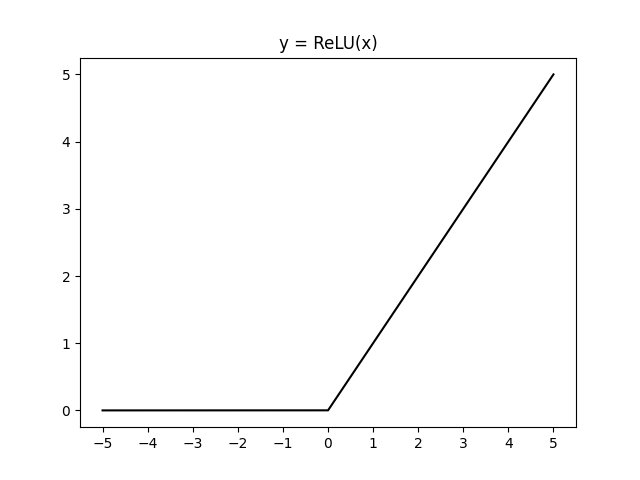
\includegraphics[scale=0.5]{/diagrams/relu}
\caption{Graph of ReLU function}
\end{figure}
\[tanh(x) = \frac{e^{x} - e^{-x}}{e^{x}+e^{-x}}\]
\begin{figure}[H]
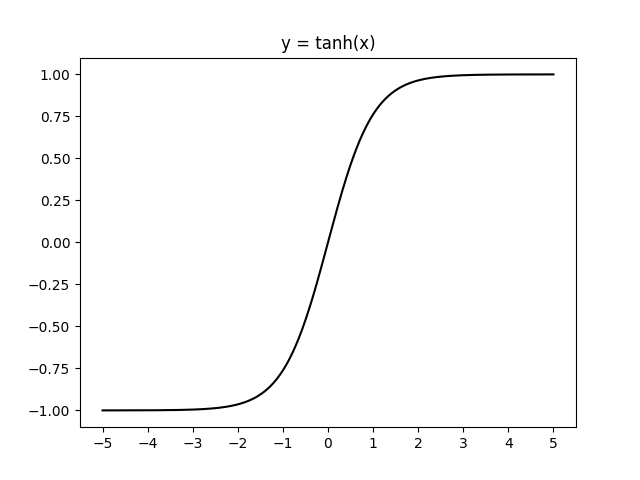
\includegraphics[scale=0.5]{/diagrams/tanh}
\caption{Graph of tanh function}
\end{figure}
\end{centering}

\subsection*{2.2 Computational Background}

For the computational background, we will look at some algorithms inherent to the solution of our problem, and machine learning as a whole.\\

First, we look at two stochastic gradient descent algorithms, called ADAM and RMSProp. Adam is just one of many available algorithms for this purpose, but is experimentally shown to provide better results than other contemporary algorithms (Kingma \& Ba, 2017). RMSProp (full name: root mean square propagation) is an "adaptive learning rate [method]", which is an "extension of Stochastic Gradient Descent and... the foundation of Adam" (Huang 2020). Both of these options work very similarly to other numerical gradient descent algorithms, by iteratively updating some parameter, to minimize some function. In a machine learning application, this parameter is one of the model parameters (recall, weights and biases), and the function is the model loss function. In the specific case of an adaptive learning rate method, of which these both are, the learning rate changes over the course of the running.\\\\

Second, is kind of an algorithm, but can also be thought of as a simple process. Backpropagation, as an algorithm, is repeated use of the chosen stochastic gradient descent algorithm. It is applied first to the last layer of the model, optimizing the loss function based on the very last set of weights and biases we get to tweak. Then, we backpropagate, applying this algorithm to the next layer back in the chain. Then the next layer back, and so on, until we have minimized the loss function for every weight and bias involved.\\\\

We will now make a quick note, for the promised explanation of parameters versus hyperparameters. A parameter, with respect to a machine learning model, is something that directly influences the output. This means that, if we were to find a general mathematical expression for the loss function, these parameters would be in there. A hyperparameter is a parameter of the model itself. These involve learning rate, number of filters in a convolutional layer, stride size, neighbourhood size, et cetera. These hyperparameters influence the accuracy of the model, but they do not directly influence the output. The ``training'' of a machine learning model refers to applying backpropagation to optimize the loss function with respect to some training dataset.

\subsection*{3 Methodology}
\subsection*{3.1 Original Architecture}
To explain the methodology for classifying images from the MNIST dataset, we begin by discussing how the model takes input, and describing that input. \\

The MNIST dataset consists of $70000$ $28\times 28$ images, depicting handwritten numbers. These images, as noted previously, are centred and padded with whitespace. We encode these images as tensors in three dimensions: length, width, and the intensities of the RGB channels. So any image can be encoded in a tensor of dimension $(n, n, 3)$. We can further simplify this dimension by grayscaling the images, resulting in a square matrix of dimension $(n, n)$, where each image corresponds to the intensity of a pixel. By doing this, we can write our model as a function $f: M_{n,n} \rightarrow  \{0,1,\cdots,9\}$.\\

Our machine learning model utilizes a convolutional neural network (otherwise known as a CNN). This is a neural network that focuses on image recognition through the use of convolutional layers to detect patterns across images. This structure is ideal for our problem, because it is specifically an architecture meant to deal with images. Our specific (original) structure is as follows. We start with the image encoded into a tensor as described, and that is provided as input to a convolutional layer. This convolutional layer has six filters, a neighbourhood size of five, and a stride of one. We connect this to a max-pooling layer with a neighbourhood size of two, and again a stride of one. The layers are then flattened to a dense layer of sixty-four neurons. We connect this to a final dense layer of ten neurons, which provides the output. Note that the convolutional layer and first dense layer use rectilinear activation functions, and the output layer uses a softmax activation function to produce a final probability distribution.
\begin{figure}[H]
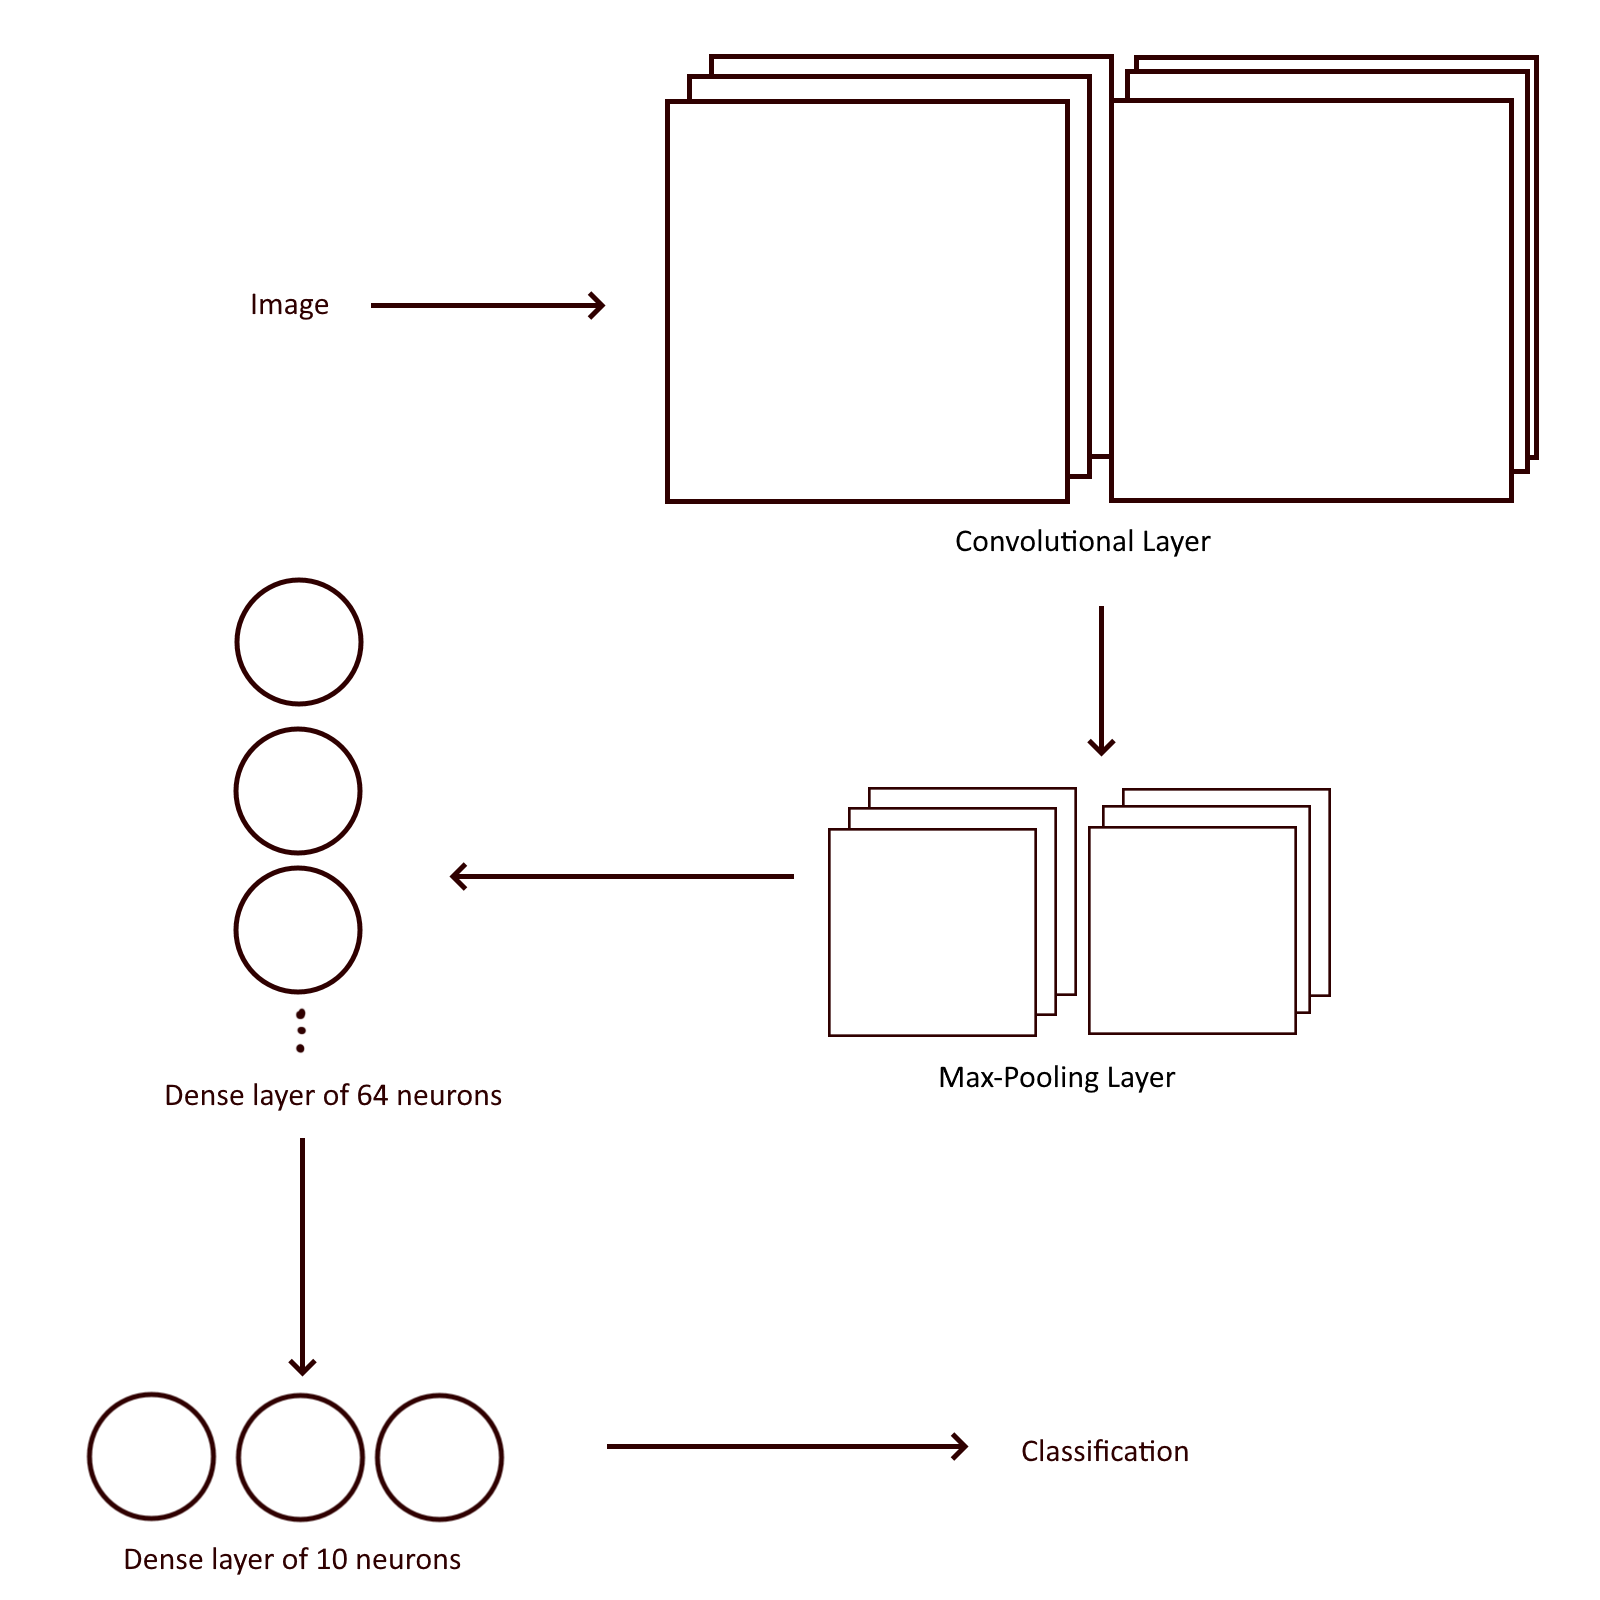
\includegraphics[width=\textwidth]{/diagrams/modelarchitecture}
\caption{The original model architecture}
\end{figure}

Even if the model is competently structured, a new problem of overfitting can arise during the training process. Overfitting describes the scenario where a model is trained too extensively on a chosen training dataset, and so performs suboptimally on data outside of that training dataset. Cross-validation is a technique used to prevent this; the specific method we use is called $k$-fold cross-validation. $k$-fold cross-validation works by splitting the training data allocated to each training step (also called an epoch) into $k$ subsets, then training the model on all but one of these subsets. The final subset is then used to validate the performance of the model. When a chosen metric - usually accuracy - begins declining during validation steps, the training is stopped.

\subsection*{3.2 Evaluation and Assessment Metrics}
We use two metrics to evaluate the performance of our model. The first is accuracy, which is the ratio of true guesses to total guesses. This tends to be a good metric, because of how intuitive it is. A given percentage accuracy can intuitively be interpreted as a percentage of correct answers. The second metric is a confusion matrix. This is a kind of matrix used to visualize the guesses of the model and the true value of the image. One axis of the confusion matrix represents the true label of  the input image, and the other axis represents the predicted label. The entry $(i, j)$ of this matrix is the total number of times true label $i$ was predicted to have label $j$ by the model. The ideal confusion matrix is a perfectly diagonal matrix. In practice, because a perfect model is nearly impossible, we instead try to make the matrix as sparse as possible.

\subsection*{3.3 Improving the Model}
The original model architecture, when training it multiple times, tended to receive accuracy scores of around $97\%$. The confusion matrix was less than ideal, pointing towards some critical areas of confusion, where $7$'s and $8$'s mapped to $2$ and $3$ more than should have been expected. So obviously, there was room for improvement, and we wanted to seize upon it.
\begin{figure}[H]
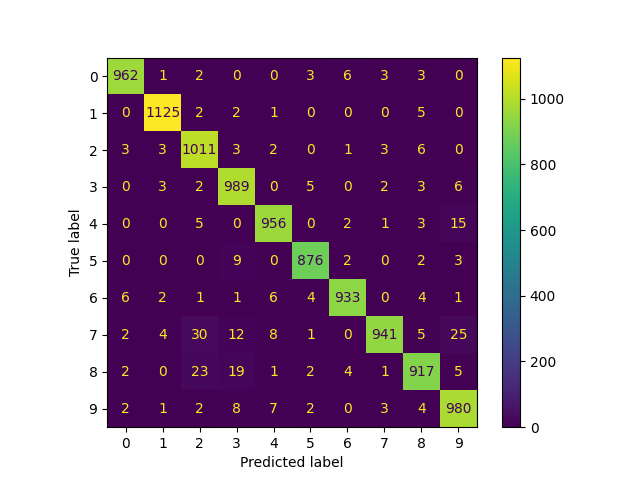
\includegraphics[width=\textwidth]{/exp/default_confusionmatrix}
\caption{The original model's confusion matrix}
\end{figure}

There were three approaches we planned to take to this end. First, we tried a brute-force approach of testing every possible combination of hyperparameters. This approach was temporally infeasible, as the costs of the experiments grew exponentially. Rough calculations yielded an estimated time to complete of two weeks, provided we co-opted every phone, laptop, and desktop owned by four separate people for the entire length of that time. So we looked towards more efficient solutions, that weren't guaranteed to find the optimal set of parameters.\\

The first of these approaches, we refer to as the naive approach. In this approach, we isolated each parameter from the base model, and iterated over it alone. An example of one of these experiments can be seen below:
\begin{figure}[H]
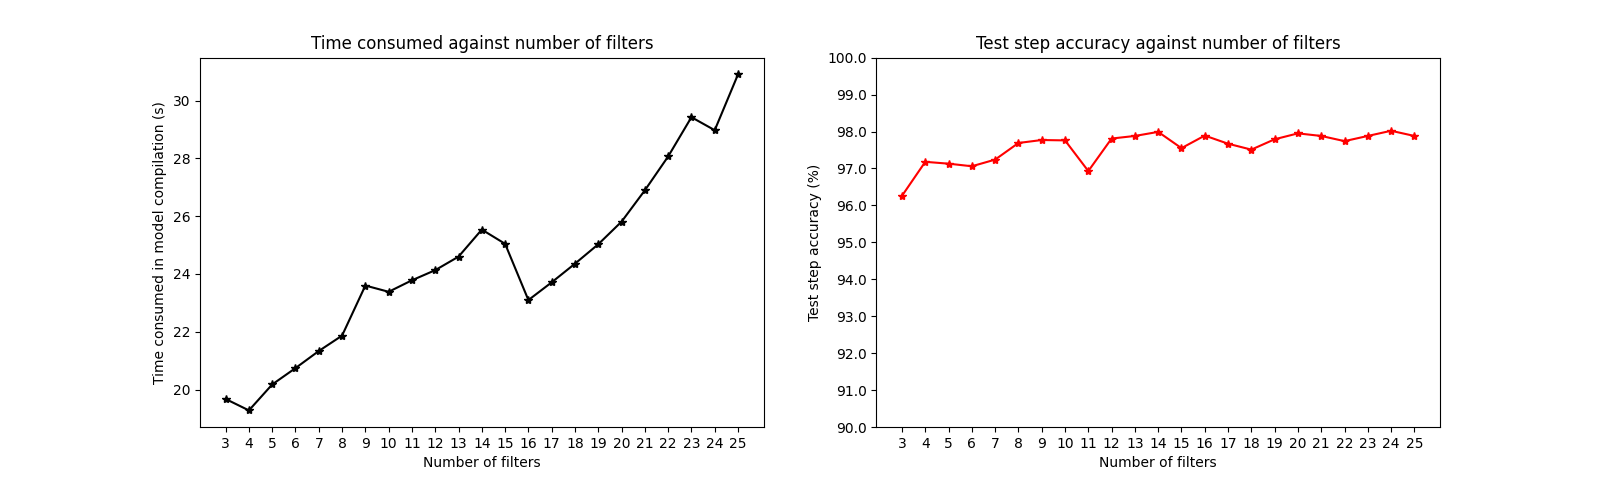
\includegraphics[width=\textwidth]{/exp/filter_3-25}
\caption{An experiment testing different filter counts}
\end{figure}
As can be seen in this figure, the maximum accuracy comes from a filter count around fourteen to sixteen. For the naive approach, we selected exactly fourteen for the filters. We will discuss a full list of hyperparameters later.\\

For the second reasonable approach, we refer to it as the greedy approach. For this method, we isolated a hypothesized most important hyperparameter from the base model (epochs) and then use the same iterative approach to optimize based on that. The key difference to this approach is that we fixed the first parameter before moving on to the second. This models the greedy programming strategies of taking the optimal local solution at every given step, and is why we refer to this as the greedy model.

\pagebreak
\subsection*{3.4 The New Models}
The full list of hyperparameters that were adjusted is as follows:
\begin{center}
\begin{tabular}{|c|c|c|c|}
\hline
$\frac{Model}{Parameter}$ & Original & Naive & Greedy\\
 & & & \\
Epoch Count & 5 & 15 & 15\\
Activation Function & ReLU & tanh & ReLU\\
Optimizer Algoritm & Adam & RMSProp & RMSProp\\
Convolutional Filters & 6 & 14 & 16\\
Convolutional Neighbourhoods & 5 & 7 & 7\\
Max-Pooling Neighbourhoods & 2 & 2 & 3\\
\hline
\end{tabular}
\end{center}
Though arrived at from slightly different pathways, the naive and greedy models both have a very similar set of hyperparameters. In particular, we should note that the epoch count is expected to be exactly the same, since that was the first parameter looked at. The structuring of the table is also important, in that this is the order we hypothesized would be most important for the greedy model.
\subsection*{4 Discussion}
\subsection*{4.1 Model Results}
\begin{figure}[H]
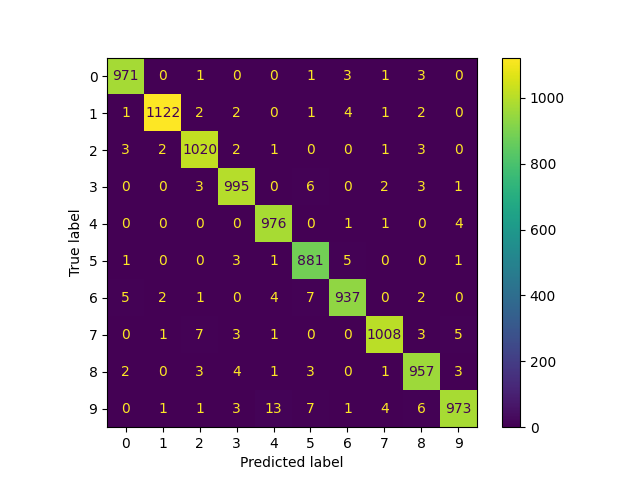
\includegraphics[width=\textwidth]{/exp/naive_confusionmatrix}
\caption{The confusion matrix for the naive model}
\end{figure}
\begin{figure}[H]
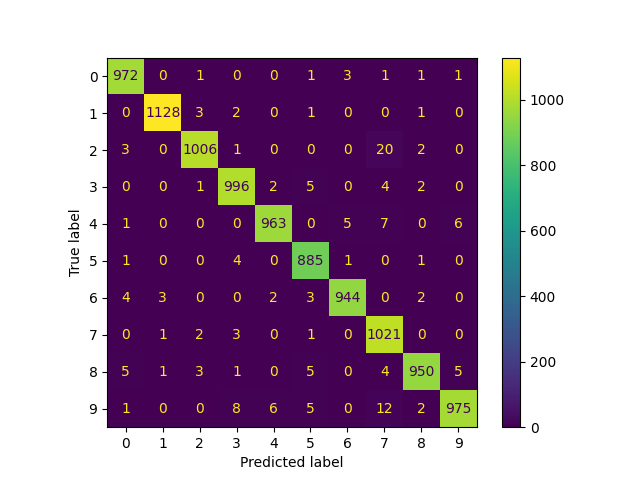
\includegraphics[width=\textwidth]{/exp/greedy_confusionmatrix}
\caption{The confusion matrix for the greedy model}
\end{figure}
These two models both score accuracy in the test step around $98.5\%$. As can be gleaned from their respective confusion matrices, there is (on average) less confusion. The two models, despite nearly identical accuracy, make mistakes in different places. For example, notice how the naive model tends to make scattered mistakes, whereas the greedy model displays particular repeat errors mapping images incorrectly to $7$. It becomes hard to describe one of these models as ``better'' than the other, since there is no context applied to the problem. Although, both, clearly, are improvements over the original model.

\subsection*{4.2 Limitations of the Data}
This $~98.5\%$ is not quite a hard limit on the accuracy, but we hypothesize that it isn't far off from one. In this section, we will discuss how some of the MNIST data itself poses an obstacle to the training for any potential CNN.
\begin{figure}[H]
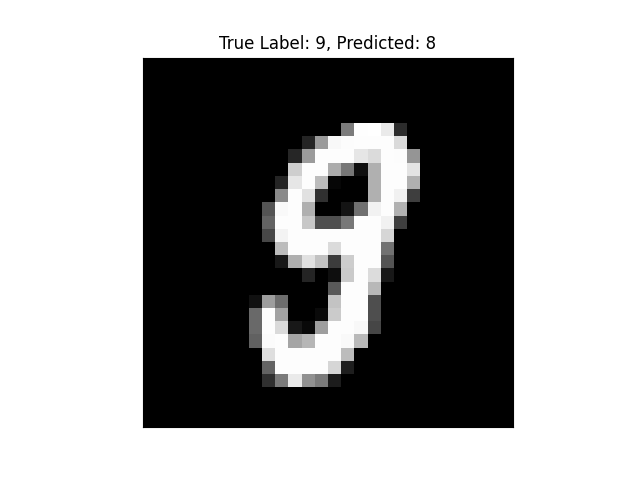
\includegraphics[width=\textwidth]{/exp/t9p8}
\caption{Image with true label: 9 Greedy prediction: 8}
\end{figure}
In this particular image, a human eye \textit{can} usually recognize the digit as a nine. However, the model does not. The gap in the arm of the nine is very small, in fact, smaller than the convolutional layer's neighbourhood. This, in a manner of speaking, hides the gap from the model. It shouldn't come across as infeasible for the model to be confused by this image. The way to combat this would be to add more filters and lower the neighbourhood size, but that tends to decrease performance across more typical images.
\begin{figure}[H]
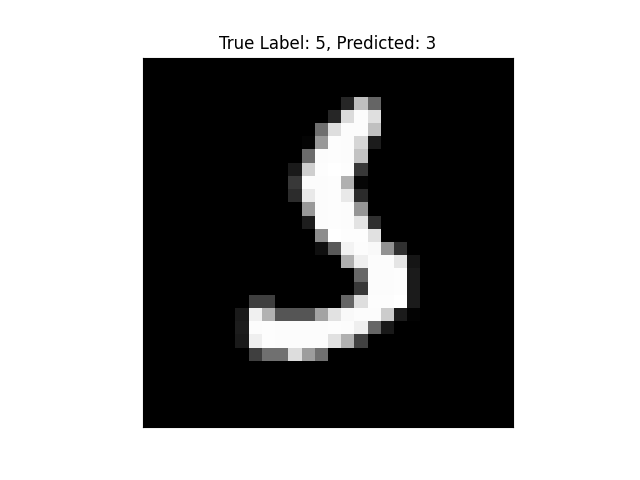
\includegraphics[width=\textwidth]{/exp/t5p3}
\caption{An image misclassified by the greedy model}
\end{figure}
In this image, we see a very confusing digit. We contend that to most human eyes, it is hard to determing exactly which number this is supposed to be. In fact, please attempt this as an exercise before reading further. Make a decision about what \textit{you, the reader} would classify this image as.\\\\
We will provide the answer at the end of this paragraph, after a moment of discussion. This image is confusing. There is an arch at the bottom that looks reminiscent of both a $5$ and $3$, but it lacks the other distinguishing feature of either number. Namely, the hat of the $5$ or the twin top-arch of the $3$. This image is a very good example of why we believe any model solving this problem does not have a theoretical maximum accuracy of $100\%$. There are outliers like this, which cannot reliably be classified without overfitting on purpose.\\\\
As promised, it was actually a $5$, and misclassified as a $3$. Either one of those predictions we take as reasonable, from a human.
\subsection*{5 Conclusion}
In this report, we have detailed a strong architecture and set of hyperparameters that together do a good job balancing training costs and performance. It has not been previously mentioned, as training time doesn't tend to be considered as important as the evaluation metrics, but these models take less than a minute to train. This low cost and high performance allow this specific model to be used well in many different kinds of applications, and easily replicated.\\\\
In this report, we have also seen why models do not usually reach $100\%$ test accuracy, and why a model with perfect test accuracy should be carefully inspected to ensure it has not been horribly overfitted. Data sets usually contains outliers and noise, and any model that fits well to outliers and noise is a bad model. It is instead preferable to achieve an almost perfect score, retaining a capacity for generalization.\\\\
\subsection*{6 Code Source}
All notes, figures and code created during the process of this project can be found at the following link:\\
https://github.com/TravisDurrantOTU/ml-project
\pagebreak
\subsection*{Citations}
\begin{hangparas}{0.5 in}{1}
Brownlee, J. (2020, December 22). A gentle introduction to cross-entropy for Machine Learning. MachineLearningMastery.com. https://machinelearningmastery.com/cross-entropy-for-machine-learning/\newline

Huang, J. (2020). RMSPROP. Cornell University Computational Optimization Open Textbook - Optimization Wiki. https://optimization.cbe.cornell.edu/index.php?title=RMSProp \newline

Kingma, D. P., \& Ba, J. (2017, January 30). Adam: A method for stochastic optimization. arXiv.org. https://arxiv.org/abs/1412.6980\newline

Nielsen, M. A. (2019, January 1). Neural networks and deep learning. \newline http://neuralnetworksanddeeplearning.com/index.html\newline

Parnami, A., \& Lee, M. (2022, March 7). Learning from few examples: A summary of approaches to few-shot learning. arXiv.org. https://arxiv.org/abs/2203.04291\newline
\end{hangparas}
\pagebreak
Contributions made have been equally the product of work undertaken by Travis Durrant and Timothy Weathers


\end{document}